\documentclass[]{article}
\usepackage{graphicx}
\graphicspath{ {media/} }
\usepackage{float}
\usepackage{subcaption}
\usepackage[margin=1.2in]{geometry}

%opening
\title{Traffic Sign Project Report}

\begin{document}

\maketitle

\section{Project Goal}
The goal of this project is to build a convolutional neural network to classify traffic signs in the German Traffic Sign dataset\cite{Stallkamp-IJCNN-2011}, and evaluate its performance.

\section{Data Exploration}
The dataset consists of three subsets.

\begin{center}
	\begin{tabular}{c | c | c | c}
		\hline
		& Training & Validation & Test \\ \hline
		Example Count & 34799 & 4410 & 12630 \\ \hline
	\end{tabular}
\end{center}

The images in the dataset are  in 32x32x3 RGB format. The total number of sign classes is 43.

We first verify that the class label distribution in each subset are consistent. See Figure \ref{fig:comp} for a bar chart of class label count per subset. As we can see, the classes are not distributed evenly, which might cause some labels to be predicted more accurately later on, but the distribution is consistent in all three subsets, so evaluation with the validation and test sets should properly reflect model performance.

We also check if the colour distribution is consistent in three subsets. in Figure \ref{fig:colour} we see that the RGB distribution is consistent in all three datasets.

\begin{figure}[p]
	\centering
	\begin{subfigure}{0.5\textwidth}
		\centering
		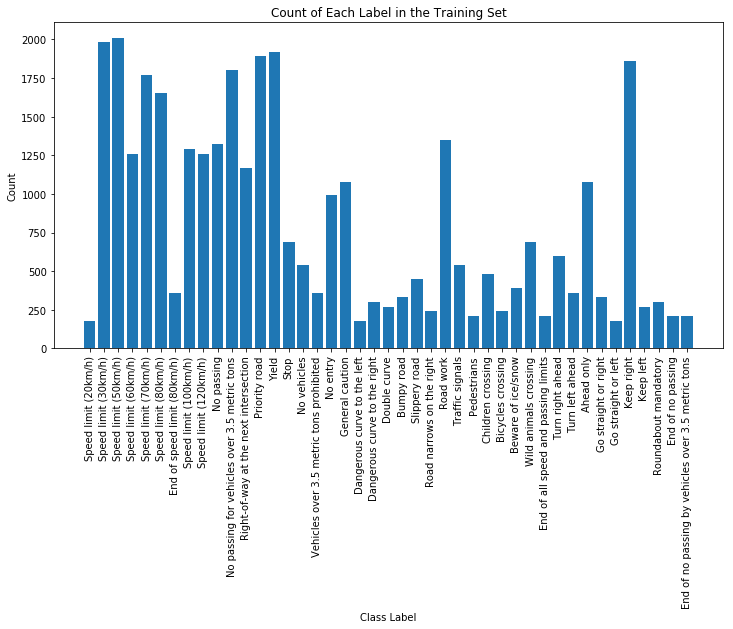
\includegraphics[width=\textwidth]{balance}
	\end{subfigure}%
	\begin{subfigure}{0.5\textwidth}
		\centering
		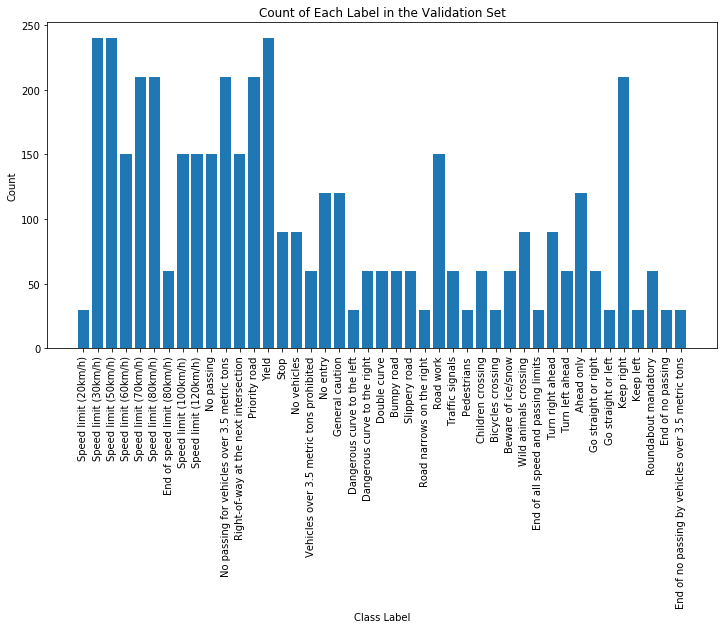
\includegraphics[width=\textwidth]{balance2}
	\end{subfigure}
	\begin{subfigure}{0.5\textwidth}
		\centering
		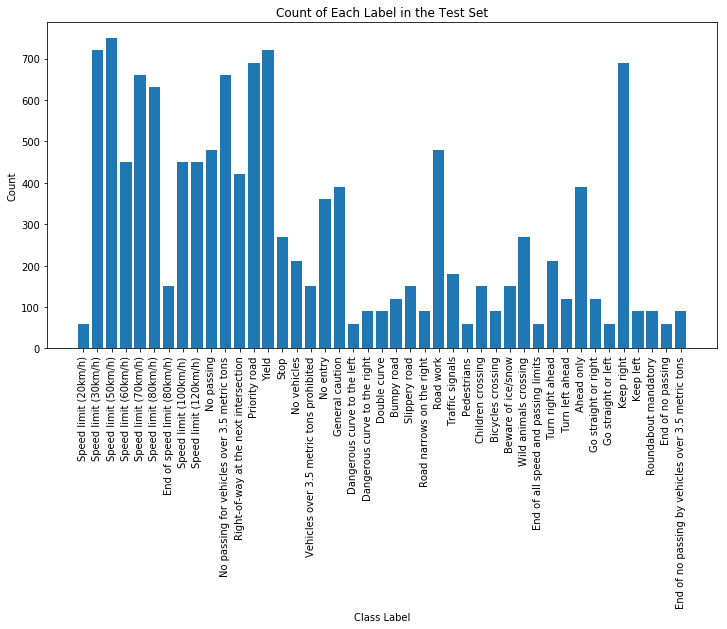
\includegraphics[width=\textwidth]{balance3}
	\end{subfigure}
	\caption{Distribution of Class Labels in Each Subset}
	\label{fig:comp}
	
\end{figure}

\begin{figure}[p]
	\centering
	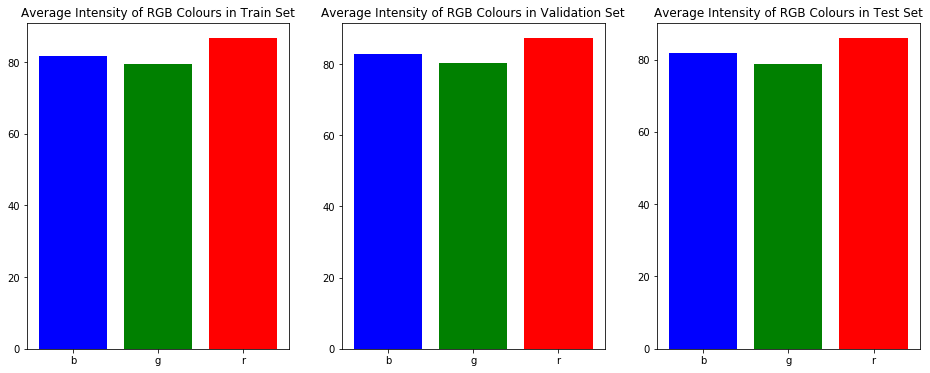
\includegraphics[width=0.8\textwidth]{cd}
	\caption{Distribution of RGB colours in Each Subset}
	\label{fig:colour}
\end{figure}

\section{Image Preprocessing}
Before we train our network on the images, we first need to preprocess the data to provide a normalised input for the network. the easiest approach is to subtract the mean from the images half the range, but we observed that some images have larger range of colour and brightness variations than others, therefore a per-image normalisation is used to ensure consistent variation ranges for all images.

We also perform a data augmentation step for all training data by adding some random noise to the images. During training, before the network consumes the input, the input images are randomly perturbed in hue, brightness, saturation and contrast by a small amount. This helps increase the robustness of the network and reduce overfitting. We do not expand the original training set. Instead, we perform this perturbation each passthrough so that each epoch, the network trains on slightly different versions of each training example. Luckily, we can incorporate this step into the Tensorflow computation graph.

\newpage
\section{Model Architecture}

Our network uses the following architecture:

\begin{center}
	\begin{tabular}{c | c | c | c | c}
		\hline
		Layer No. & Layer Type & Dimensionality & Activation & Note \\ \hline
		1 & Conv2D & 16x[3, 3] & ReLU & Valid Padding, L1 Regularisation (0.1) \\ \hline
		2 & MaxPooling & [2, 2] & None & Stride=2 \\ \hline
		3 & Conv2D & 32x[3, 3] & ReLU & Valid Padding, L1 Regularisation (0.1) \\ \hline
		4 & MaxPooling & [2, 2] & None & Stride=2 \\ \hline
		5 & Dense & 512 & ReLU & Batch Normalisation \\ \hline
		6 & Dropout & - & None & Drop Rate=0.7 \\ \hline
		7 & Dense & 512 & ReLU & Batch Normalisation \\ \hline
		8 & Dropout & - & None & Drop Rate=0.7 \\ \hline
		9 & Dense & 43 & Linear / Softmax & Output \\ \hline
	\end{tabular}
\end{center}

The computation graph has an auxiliary boolean input \textit{is\_training} to inform the network whether to perform noise adding and dropout in forward passthrough. The whole forward pass architecture can be seen in Appendix Figure \ref{fig:arch}.

[3, 3] kernels are found to perform better than [5, 5] kernels, likely due to the fact that the details in traffic signs exhibit difference on a small scale. L1 regularisation here is used to induce sparsity in the convolution kernels so they focus on different aspects of the input image. A pair of high dimensional dense layers are used in conjunction with a high dropout rate to achieve a balance between expressiveness and overfitting control. Batch normalisation is employed to combat rapid overfitting during training, in addition to the high dropout rate. An additional convolutional layer is found to be contributing little to the validation accuracy, so only two convolutional layers are used in this model.

\section{Training and Evaluation}

The network is trained on the training dataset with a batch size of 32 over 20 epochs. Input images are shuffled each epoch. The network is trained with an Adam optimiser with a learning rate of $5 \times 10^{-4}$. Loss and accuracy are evaluated per epoch on both the training and validation set. The training vs validation loss over training steps is shown in figure \ref{fig:loss}.

\begin{figure}[H]
	\centering
	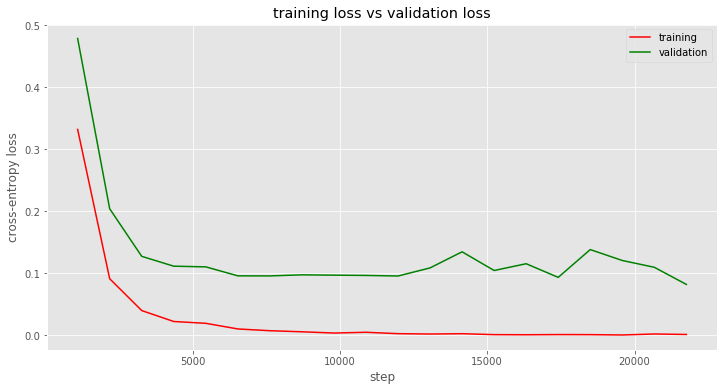
\includegraphics[width=0.65\textwidth]{loss}
	\caption{training vs validation loss}
	\label{fig:loss}
\end{figure}

The final training accuracies are \textbf{99.96\%} on the training set and \textbf{98.18\%} on the validation set.
The network achieves \textbf{96.22\%} accuracy on the test dataset.

\section{Performance Analysis}

To analyse the performance of the network in more detail, we acquired five new German traffic sign images from Google Image Search and predicted their top 5 labels with the classifier. Here are the results:

\begin{figure}[H]
	\centering
	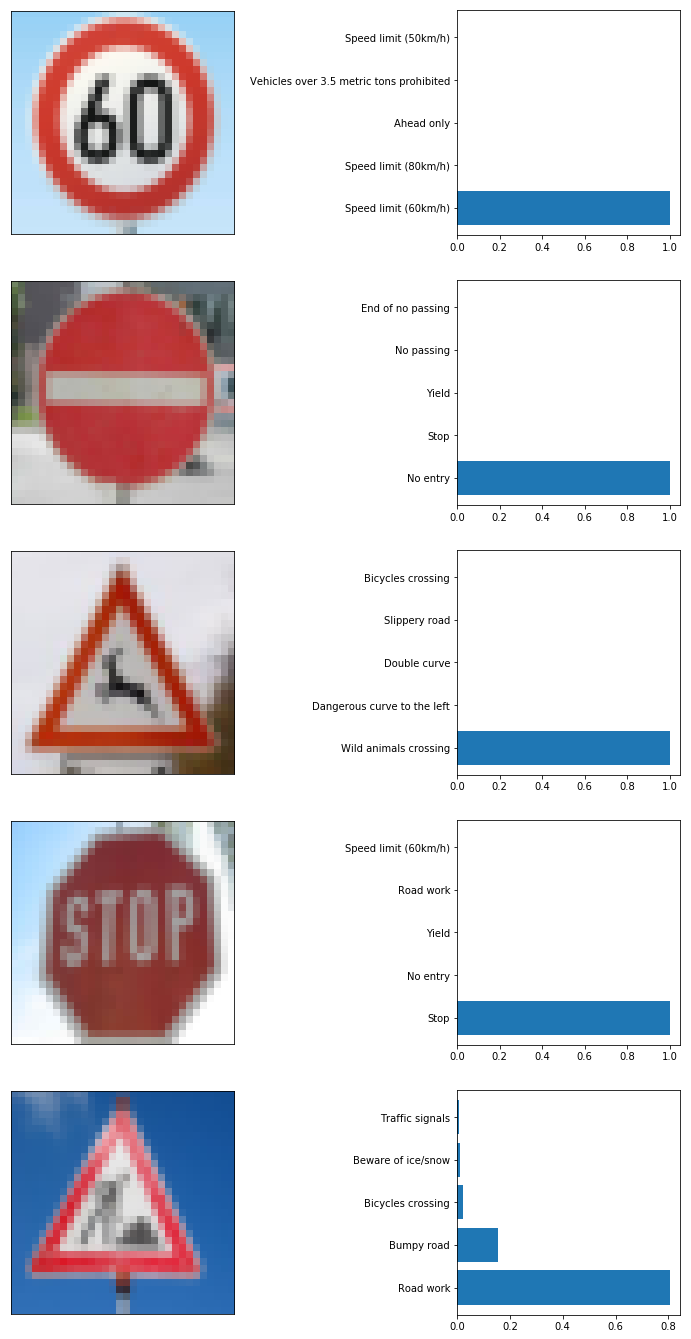
\includegraphics[width=0.6\textwidth]{newpred}
	\caption{Prediction with New Images}
	\label{fig:newpred}
\end{figure}

As we see, the network is able to provide correct predictions for all images. In addition, it is able to provide "confident" predictions for all images except "Road Work". However, we will show later that the softmax probability is not a good measure of the network's confidence.

Since the network is able to correctly classify all new images, we have to examine the misclassified images in the test dataset to figure out how it behaves when it fails to classify correctly. Here are some of the examples of misclassification:

\begin{figure}[H]
	\centering
	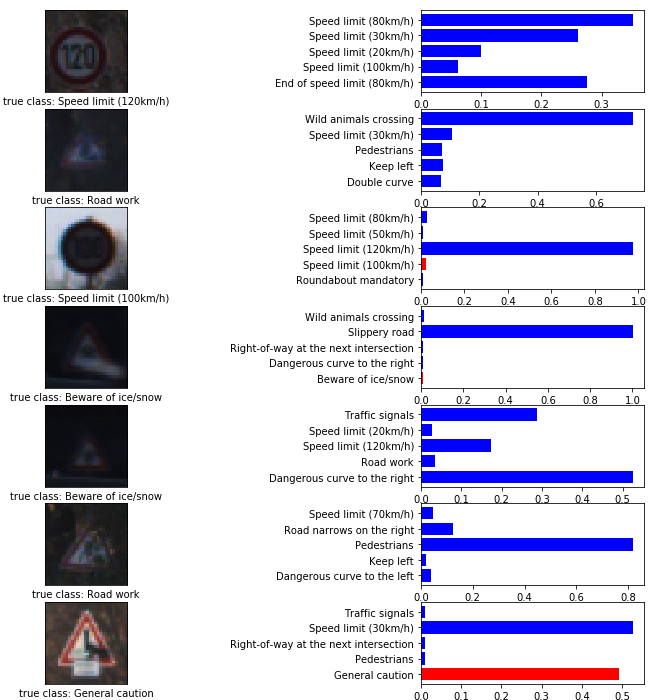
\includegraphics[width=0.6\textwidth]{wrong_small}
	\caption{Misclassifications}
	\label{fig:mis}
\end{figure}

Here, we see that in some cases, the softmax probability reflects the uncertainty of the classifier (such as the first image), whereas in some other cases, even though the image is so blurry that eeven a human cannot easily label it, the network provides an extremely "confident" output that is quite wrong. Is there another way to estimate the uncertainty of the network? Recall that we do not include the noise adding and dropout steps in the evaluation pipeline. One idea is to add these stochastic elements back into the network, let it predict with uncertainty, and examine a sample of its prediction to gauge its confidence. As an example, we take the sixth image ("Road work") and run it through the network 10000 times with noise and dropout enabled (Figure \ref{fig:sto}).

As we see in the bar chart, even though the network is still unable to guess the correct label, the distribution of different labels in the sample is closer than the softmax probabilities to where the uncertainty should be.

\begin{figure}[H]
	\centering
	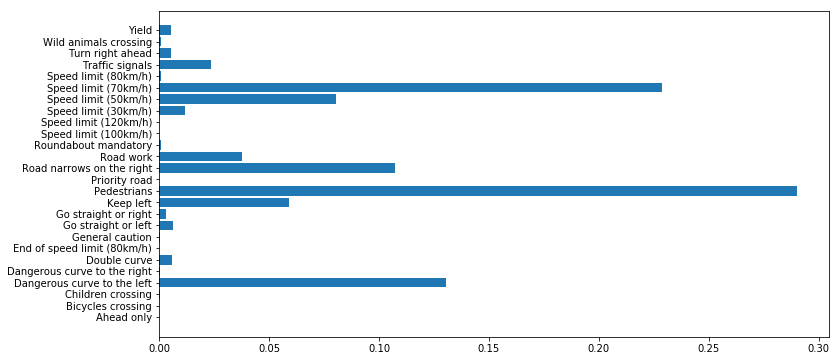
\includegraphics[width=0.8\textwidth]{rw}
	\caption{Stochastic Prediction Sample}
	\label{fig:sto}
\end{figure}

We also calculate the per-class percision and recall in Appendix Table \ref{tbl:pnr}. The classes with the worst precision are \textbf{Speed limit (20km/h), Pedestrians and Beware of ice/snow}, and the classes with the worst recall are \textbf{Speed limit (120km/h), Pedestrians and Dangerous curve to the right}. Overall, the network is struggling the most with the class \textbf{Pedestrians}. We wonder why this is the case. Here are the classes that \textbf{Pedestrian} images are most commonly classified as:

\begin{figure}[H]
	\centering
	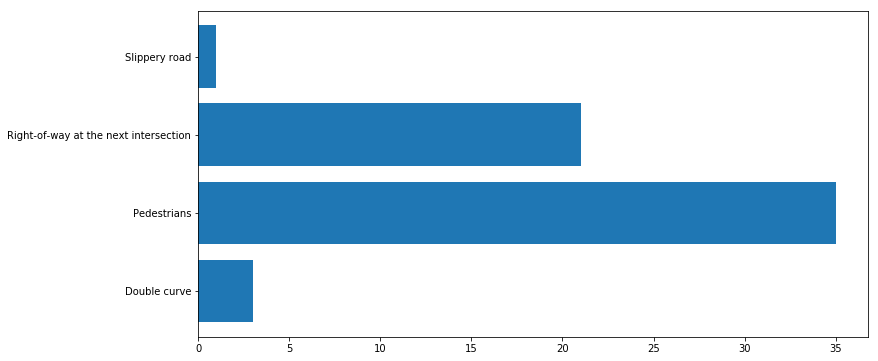
\includegraphics[width=0.7\textwidth]{ped}
	\caption{Pedestrian Class Prediction Outcome}
	\label{fig:ped}
\end{figure}

It appears that the network frequently confuses \textbf{Pedestrian} with \textbf{Right-of-way at the next intersection}, which is indeed very similar in appearance. At the given image resolution, it is even difficult for humans to distinguish between the two.

\section{Activation Visualisation}

Neural networks are often treated as black boxes, as the precise function of each layer and each node is difficult to pinpoint. However, sometimes it is possible to crudely estimate the function of a convolution kernel in a CNN by examining its activation patterns. Here, we visualise the mean activations of our convolutional layers for all circular-plate signs versus triangular-plate signs. We focus on the first convolutional layer, as the second layer is harder to interpret.

\begin{figure}[H]
	\centering
	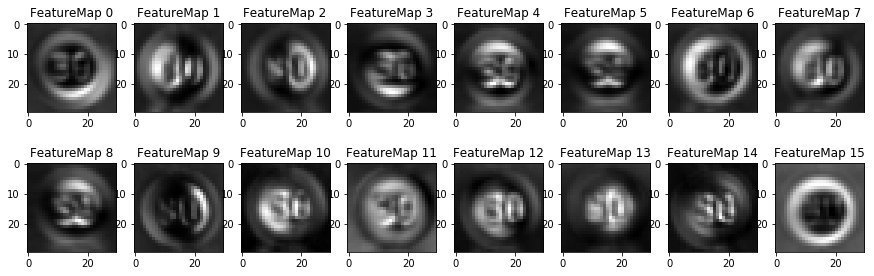
\includegraphics[width=0.7\textwidth]{fm1c}
	\caption{Conv Layer 1 for Circular Plates}
	\label{fig:c1}
\end{figure}

\begin{figure}[H]
	\centering
	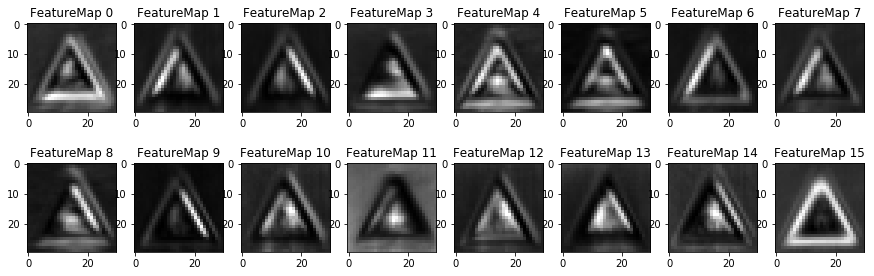
\includegraphics[width=0.7\textwidth]{fm1t}
	\caption{Conv Layer 1 for Triangular Plates}
	\label{fig:t1}
\end{figure}

Notice that in both cases, the feature map 15 in the first convolution layer is always detecting the coloured stripe / ring around the sign, regardless of the shape of the sign, whereas feature map 13 in the first convolution layer always focuses on the interior of the sign. The different kernels focus on different aspects of the input images and create more meaningful features for the following layers.

\section{Further Improvements}

The current network architecture and data pipeline are not perfect and may still be improved. For example, the data augmentation step only used per-pixel noise-adding. By utilising other transformations such as rotation and translation, we may further improve the performance. The network also appears to struggle a little bit with some off-centre images or smaller signs, so some form of multi-scale solution (such as parallel convolutional layers of different kernel sizes) can be helpful. Also, the training curve of the network shows that the validation loss has not yet stablised or "bounced back", so we may not have reached optimality during training yet. By tweaking the training parameters, we may be able to reach a better optimal point.

\bibliographystyle{acm}
\bibliography{report}

\newpage
\section*{Appendix}

\begin{figure}[H]
	\centering
	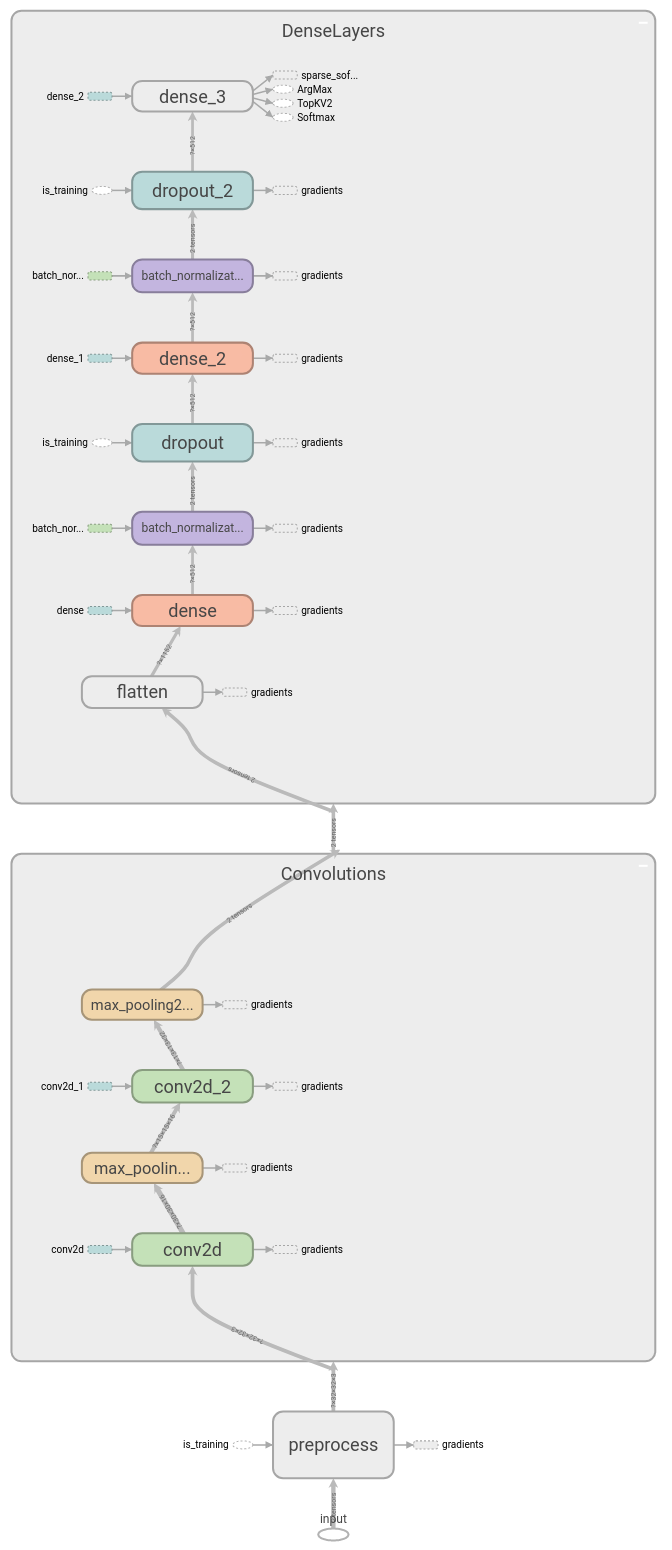
\includegraphics[width=0.55\textwidth]{arch}
	\caption{Network Architecture}
	\label{fig:arch}
\end{figure}

\begin{table}[]
	\centering
	\caption{Per-class Precision and Recall}
	\label{tbl:pnr}
	\resizebox{\textwidth}{!}{%
		\begin{tabular}{lllllll}
			row & label\_ID & true\_label & precision                                         & recall   & precision\_rank & recall\_rank    \\ \hline \hline
			0         & 0           & Speed limit (20km/h)                              & 0.566667 & 1.000000        & 42           & 0  \\ \hline
			1         & 1           & Speed limit (30km/h)                              & 0.988889 & 0.966079        & 15           & 26 \\ \hline
			2         & 2           & Speed limit (50km/h)                              & 0.980000 & 0.965834        & 18           & 27 \\ \hline
			3         & 3           & Speed limit (60km/h)                              & 0.935556 & 0.972286        & 32           & 24 \\ \hline
			4         & 4           & Speed limit (70km/h)                              & 0.966667 & 0.990683        & 23           & 12 \\ \hline
			5         & 5           & Speed limit (80km/h)                              & 0.953968 & 0.909228        & 28           & 35 \\ \hline
			6         & 6           & End of speed limit (80km/h)                       & 0.820000 & 0.991935        & 38           & 10 \\ \hline
			7         & 7           & Speed limit (100km/h)                             & 0.882222 & 0.985112        & 35           & 15 \\ \hline
			8         & 8           & Speed limit (120km/h)                             & 0.993333 & 0.809783        & 8            & 42 \\ \hline
			9         & 9           & No passing                                        & 0.987500 & 0.979339        & 16           & 22 \\ \hline
			10        & 10          & No passing for vehicles over 3.5 metric tons      & 0.975758 & 0.993827        & 22           & 7  \\ \hline
			11        & 11          & Right-of-way at the next intersection             & 0.992857 & 0.892934        & 9            & 38 \\ \hline
			12        & 12          & Priority road                                     & 0.995652 & 0.984241        & 5            & 16 \\ \hline
			13        & 13          & Yield                                             & 0.997222 & 0.993084        & 3            & 8  \\ \hline
			14        & 14          & Stop                                              & 0.996296 & 1.000000        & 4            & 3  \\ \hline
			15        & 15          & No vehicles                                       & 1.000000 & 0.981308        & 2            & 20 \\ \hline
			16        & 16          & Vehicles over 3.5 metric tons prohibited          & 0.993333 & 1.000000        & 7            & 2  \\ \hline
			17        & 17          & No entry                                          & 0.991667 & 1.000000        & 12           & 1  \\ \hline
			18        & 18          & General caution                                   & 0.935897 & 0.973333        & 31           & 23 \\ \hline
			19        & 19          & Dangerous curve to the left                       & 1.000000 & 0.983607        & 1            & 17 \\ \hline
			20        & 20          & Dangerous curve to the right                      & 0.977778 & 0.814815        & 20           & 40 \\ \hline
			21        & 21          & Double curve                                      & 0.855556 & 0.905882        & 36           & 36 \\ \hline
			22        & 22          & Bumpy road                                        & 0.950000 & 0.957983        & 30           & 28 \\ \hline
			23        & 23          & Slippery road                                     & 0.980000 & 0.942308        & 19           & 33 \\ \hline
			24        & 24          & Road narrows on the right                         & 0.900000 & 0.843750        & 34           & 39 \\ \hline
			25        & 25          & Road work                                         & 0.954167 & 0.950207        & 27           & 31 \\ \hline
			26        & 26          & Traffic signals                                   & 0.850000 & 0.987097        & 37           & 14 \\ \hline
			27        & 27          & Pedestrians                                       & 0.583333 & 0.813953        & 41           & 41 \\ \hline
			28        & 28          & Children crossing                                 & 0.953333 & 0.966216        & 29           & 25 \\ \hline
			29        & 29          & Bicycles crossing                                 & 0.933333 & 0.893617        & 33           & 37 \\ \hline
			30        & 30          & Beware of ice/snow                                & 0.720000 & 0.990826        & 40           & 11 \\ \hline
			31        & 31          & Wild animals crossing                             & 0.966667 & 0.981203        & 24           & 21 \\ \hline
			32        & 32          & End of all speed and passing limits               & 1.000000 & 0.937500        & 0            & 34 \\ \hline
			33        & 33          & Turn right ahead                                  & 0.995238 & 0.995238        & 6            & 6  \\ \hline
			34        & 34          & Turn left ahead                                   & 0.991667 & 0.952000        & 11           & 30 \\ \hline
			35        & 35          & Ahead only                                        & 0.992308 & 0.992308        & 10           & 9  \\ \hline
			36        & 36          & Go straight or right                              & 0.966667 & 0.983051        & 25           & 19 \\ \hline
			37        & 37          & Go straight or left                               & 0.983333 & 0.983333        & 17           & 18 \\ \hline
			38        & 38          & Keep right                                        & 0.989855 & 0.997080        & 13           & 5  \\ \hline
			39        & 39          & Keep left                                         & 0.977778 & 0.956522        & 21           & 29 \\ \hline
			40        & 40          & Roundabout mandatory                              & 0.966667 & 0.988636        & 26           & 13 \\ \hline
			41        & 41          & End of no passing                                 & 0.816667 & 1.000000        & 39           & 4  \\ \hline
			42        & 42          & End of no passing by vehicles over 3.5 metric ... & 0.988889 & 0.946809        & 14           & 32 \\ \hline
		\end{tabular}%
	}
\end{table}

\end{document}
